%\documentclass[11pt,respuestas,a4]{aleph-examen}
\documentclass[11pt,a4]{aleph-examen}
% Se puede ver la documentación aquí: 
% https://github.com/alephsub0/LaTeX_aleph-examen

% -- Paquetes adicionales 
\usepackage{aleph-comandos}
\usepackage{booktabs}
\usepackage{multicol}
\usepackage{pgfplots}

% -- Datos 
\institucion{Escuela de Ciencias Físicas y Matemática}
\carrera{Medicina Veterinaria}
\asignatura{Matemática I*}
\tema{Examen escrito no. 1}
\autor{Fernando Jiménez T.}
\fecha{Semestre 2024-2}


\logouno[0.14\textwidth]{Logos/logoPUCE_04_ac}
\definecolor{colortext}{HTML}{0030A1}
\definecolor{colordef}{HTML}{0030A1}
\fuente{montserrat}


\begin{document}

\encabezado

\section*{Indicaciones}
\begin{itemize}[leftmargin=*]
\item 
    En esta actividad se evalúa si el estudiante \textit{(Criterio 2.1) resuelve ecuaciones e inecuaciones lineales y cuadráticas de una variable utilizando las propiedades de los números reales.} 
\item
    Se encuentra prohibido el uso de cualquier fuente de información durante todo el examen.
\item
    En caso de considerar que existe un error en la pregunta o que esta se encuentra mal planteada, se debe indicar cuál es el error y justificarlo.
\item
    Todas las soluciones deben estar correctamente redactadas y explicadas.
\end{itemize}

\section*{Ejercicios}

\begin{preguntas}

%%%%%%%%%%%%%%%%%%%%%%%%%%%%%%%%%%%%%%%%
\item Complete la siguiente tabla diciendo si la ecuación es del tipo lineal, cuadrática o no lineal.\puntaje{10}
\begin{multicols}{2}
\begin{center}
    \begin{tabular}{c|c}
        Ecuación & \hspace{1cm}Tipo\hspace{1cm}  \\ \midrule
        $x^2 - 3x = 0$ &  \\[2mm]\midrule
        $2x^5  = x - 1$ & \\[2mm]\midrule
        $-5x + 1 = 0$ & \\[2mm]\bottomrule
    \end{tabular}
    
    \begin{tabular}{c|c}
        Ecuación & \hspace{1cm}Tipo\hspace{1cm}  \\ \midrule
        $\dfrac{x-7}{2} = \dfrac{2-x}{3}$ &  \\[2mm]\midrule
        $\dfrac{3}{2}x^2 - 1 = x$ & \\[2mm]\midrule
        $\sqrt{2x} - x = \sqrt{3}$ &\\\bottomrule
    \end{tabular}
\end{center}
\end{multicols}
% -----------------------------
\begin{respuesta}
\begin{center}
    \begin{tabular}{c|c}
        Ecuación & Tipo  \\ \midrule
        $x^2 - 3x = 0$ &  Cuadrática \\[2mm]\midrule
        $2x^5  = x - 1$ & No Lineal \\[2mm]\midrule
        $-5x + 1 = 0$ & Lineal \\[2mm]\midrule
        $\frac{x-7}{2} = \frac{2-x}{3}$ & Lineal \\[2mm]\midrule
        $\frac{3}{2}x^2 - 1 = x$ & Cuadrática \\[2mm]\midrule
        $\sqrt{2x} - x = \sqrt{3}$ & No lineal\\\bottomrule
    \end{tabular}
\end{center}
\end{respuesta}
%%%%%%%%%%%%%%%%%%%%%%%%%%%%%%%%%%%%%%%%
\item Resolver las siguientes ecuaciones:\puntaje{10}
\begin{multicols}{2}
    \begin{enumerate}[label=\textit{\alph*)}]
        \item $x+5 = 1 - \dfrac{1}{2}x$
        \item $\dfrac{2}{x+1} = \dfrac{1}{x}$
    \end{enumerate}
\end{multicols}
% -----------------------------
\begin{respuesta}
    \begin{enumerate}[label=\textit{\alph*)}]
        \item 
        $$
        \begin{aligned}
            x+5 &= 1 - \frac{1}{2}x \\
            (x+5) - 5 &= \left( 1 - \frac{1}{2}x \right) - 5 
            &\hspace{1cm}& \text{ restar }5 \\
            x  &= -4 - \frac{1}{2}x 
            && \text{ simplificar } \\
            x + \frac{1}{2}x &= \left(-4 - \frac{1}{2}x \right) + \frac{1}{2}x 
            && \text{ sumar } \frac{1}{2}x \\
            \frac{3}{2}x &= -4 
            && \text{ simplificar } \\
            \frac{3}{2}x \left( \frac{2}{3} \right) &= -4\left( \frac{2}{3} \right) 
            && \text{ multiplicar por } \frac{2}{3} \\
            x &= -\frac{8}{3} 
            && \text{ simplificar } \\
        \end{aligned}
        $$
        \item En este ejercicio, supondremos que $x \neq 0$ y $x \neq -1$
        $$
        \begin{aligned}
            \frac{2}{x+1} &= \frac{1}{x} \\
            \left( \frac{2}{x+1} \right) (x+1)&= \left( \frac{1}{x} \right) (x+1) 
            &\hspace{1cm}& \text{ multiplicar por }(x+1) \\
            2  &= \frac{x+1}{x} 
            && \text{ simplificar } \\
            2 (x) &= \left(\frac{x+1}{x} \right) x 
            && \text{ multiplicar por } x \\
            2x &= x+1 
            && \text{ simplificar } \\
            2x - x &= (x+1)-x 
            && \text{ restar } x \\
            x &= 1 
            && \text{ simplificar } \\
        \end{aligned}
        $$
    \end{enumerate}
\end{respuesta}
%%%%%%%%%%%%%%%%%%%%%%%%%%%%%%%%%%%%%%%%
\item Resolver las siguientes ecuaciones:\puntaje{10}
\begin{multicols}{2}
    \begin{enumerate}[label=\textit{\alph*)}]
        \item $x^2 - x - 12 = 0$
        \item $2x^4 - 6x^2 + 3= 0$
    \end{enumerate}
\end{multicols}
% -----------------------------
\begin{respuesta}
    \begin{enumerate}[label=\textit{\alph*)}]
        \item Factorando la ecuación cuadrática obtenemos la ecuación:
        $$
        (x-4)(x+3) = 0
        $$
        Aplicando, la propiedad del producto igual a cero, tenemos que
        $$
        x-4 = 0 \quad \text{o} \quad x+3 = 0
        $$
        Resolviendo cada ecuación lineal obtenemos
        $$
        x = 4 \quad \text{o} \quad x = -3
        $$
        \item Reemplazamos $t = x^2$, obteniendo:
        $$
        2t^2 - 6t + 3 = 0
        $$
        Usando la fórmula cuadrática tenemos que
        $$
        t = \frac{6 \pm \sqrt{(-6)^2 - 4(2)(3)}}{2(2)} = \frac{6 \pm \sqrt{12}}{4} = \frac{3 \pm \sqrt{3}}{2}
        $$
        Es decir,
        $$
        t = \frac{3 + \sqrt{3}}{2} \quad \text{o} \quad t = \frac{3 - \sqrt{3}}{2}
        $$
        Pero, recordemos que $t = x^2$, es decir,
        \[
        x = \sqrt{\frac{3 + \sqrt{3}}{2}} \quad \text{o} \quad x = - \sqrt{\frac{3 + \sqrt{3}}{2}} \quad \text{o}\quad x = \sqrt{\frac{3 - \sqrt{3}}{2}} \quad \text{o} \quad x = - \sqrt{\frac{3 - \sqrt{3}}{2}}. \qedhere
        \]
    \end{enumerate}
\end{respuesta}
%%%%%%%%%%%%%%%%%%%%%%%%%%%%%%%%%%%%%%%%
\item Resolver las siguientes inecuaciones y escriba la respuesta usando notación de intervalos.\puntaje{10}
\begin{multicols}{2}
    \begin{enumerate}[label=\textit{\alph*)}]
        \item $-4 < 5 - 3x$
        \item $-3 < x-4 < 2$
    \end{enumerate}
\end{multicols}
% -----------------------------
\begin{respuesta}
    \begin{enumerate}[label=\textit{\alph*)}]
        \item 
        $$
        \begin{aligned}
            -4 &< 5 - 3x \\
            (-4) - 5 &< \left( 5 - 3x \right) - 5 
            &\hspace{1cm}& \text{ restar }5 \\
            -9  &< -3x 
            && \text{ simplificar } \\
            -9 \left(-\frac{1}{3}\right) &> (-3x)\left(-\frac{1}{3}\right) 
            && \text{ multiplicar por } -\frac{1}{3} \\
            3 &> x 
            && \text{ simplificar } 
        \end{aligned}
        $$
        La solución, es el conjunto $(-\infty,3)$.
        \item 
        $$
        \begin{aligned}
            -3 &< x-4 < 2 & \\
            -3 + 4 &< (x-4) + 4 < 2+4 
            &\hspace{1cm}& \text{ sumar }4 \\
            1  &< x < 6 
            && \text{ simplificar }
        \end{aligned}
        $$
        La solución, es el conjunto $(1,6)$.\qedhere
    \end{enumerate}
\end{respuesta}
%%%%%%%%%%%%%%%%%%%%%%%%%%%%%%%%%%%%%%%%
\item Resolver las siguientes inecuaciones y escriba la respuesta usando notación de intervalos.\puntaje{10}
\begin{multicols}{2}
    \begin{enumerate}[label=\textit{\alph*)}]
        \item $x(2-3x) \leq 0$
        \item $x^2 > 2(x+6)$
    \end{enumerate}
\end{multicols}
% -----------------------------
\begin{respuesta}
    \begin{enumerate}[label=\textit{\alph*)}]
        \item Primero, notemos que la ecuación $x(2-3x) = 0$ tiene solución cuando $x = 0$ o cuando $x = \frac{2}{3}$.
        
        Usando el diagrama de signos tenemos
        \begin{center}
            \begin{tabular}{c|c|c|c}
                Intervalo & $(-\infty,0)$ & $(0,2/3)$ & $(2/3, \infty)$  \\ \hline
                Signo de $x$ & $-$ & $+$ & $+$ \\
                Signo de $(2-3x)$ & $+$ & $+$ & $-$ \\ \hline
                Signo de $x(2-3x)$ & $-$ & $+$ & $-$ \\
            \end{tabular}
        \end{center}
        Por lo tanto, $x(2-3x) \leq 0$, en los intervalos $(-\infty,0)$ y $(2/3, \infty)$. Es decir, la solución de la desigualdad es el conjunto
        $$
        (-\infty,0) \cup (2/3, \infty)
        $$
        \item Primero, pasamos todos los términos al lado izquierdo de la desigualdad, obteniendo
        $$
        x^2 - 2x - 12 > 0
        $$
        Resolvemos la ecuación $x^2 - 2x - 12 = 0$, usando la fórmula, obteniendo
        $$
        x = \frac{2 \pm \sqrt{52}}{2} = 1 \pm \sqrt{13}
        $$
        Gráficamente tenemos:
        \begin{center}
        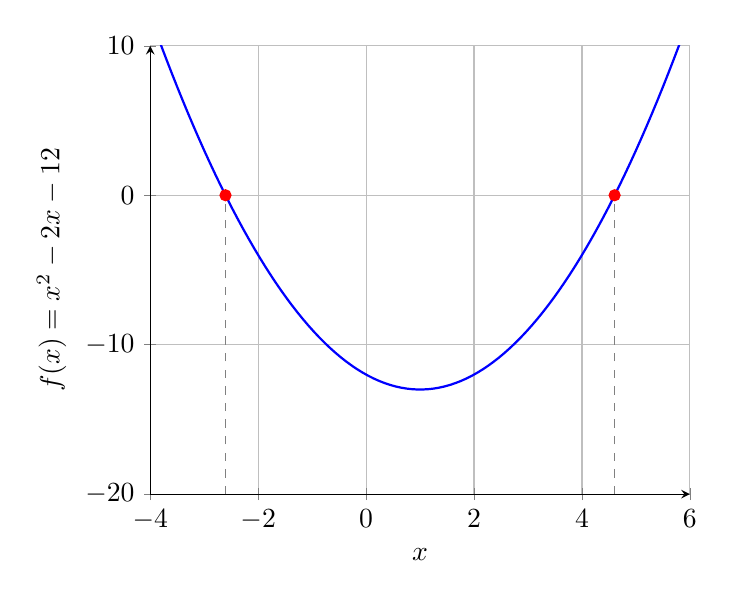
\begin{tikzpicture}
            \begin{axis}[
                axis lines = left,
                xlabel = {$x$},
                ylabel = {$f(x) = x^2 - 2x - 12$},
                ymin=-20, ymax=10, xmin=-4, xmax=6,
                grid=both,
                domain=-4:6,
                samples=100
            ]
            \addplot[color=blue, thick]{x^2 - 2*x - 12};
            \addplot[only marks, color=red, mark=*] coordinates {(1 - 13^(1/2),0) (1+ 13^(1/2),0)};

            \addplot[dashed, color=gray] coordinates {(1 - 13^(1/2),-20) (1 - 13^(1/2),0)};
            \addplot[dashed, color=gray] coordinates {(1 + 13^(1/2),-20) (1 + 13^(1/2),0)};
            \end{axis}
        \end{tikzpicture}
        \end{center}
        Notemos que la función $f(x) = x^2 - 2x - 1$ es positiva en el conjunto.
        \[
        \left(-\infty,1 - \sqrt{13}\right) \cup \left(1 + \sqrt{13}, +\infty\right).\qedhere
        \]
    \end{enumerate}
\end{respuesta}
% -----------------------------
\end{preguntas}
\end{document}